\documentclass[tikz,border=2mm]{standalone}
\usepackage{graphicx}
\usetikzlibrary{calc,angles,quotes}
\begin{document}
\begin{tikzpicture}[thick,violet]
	\node (A) {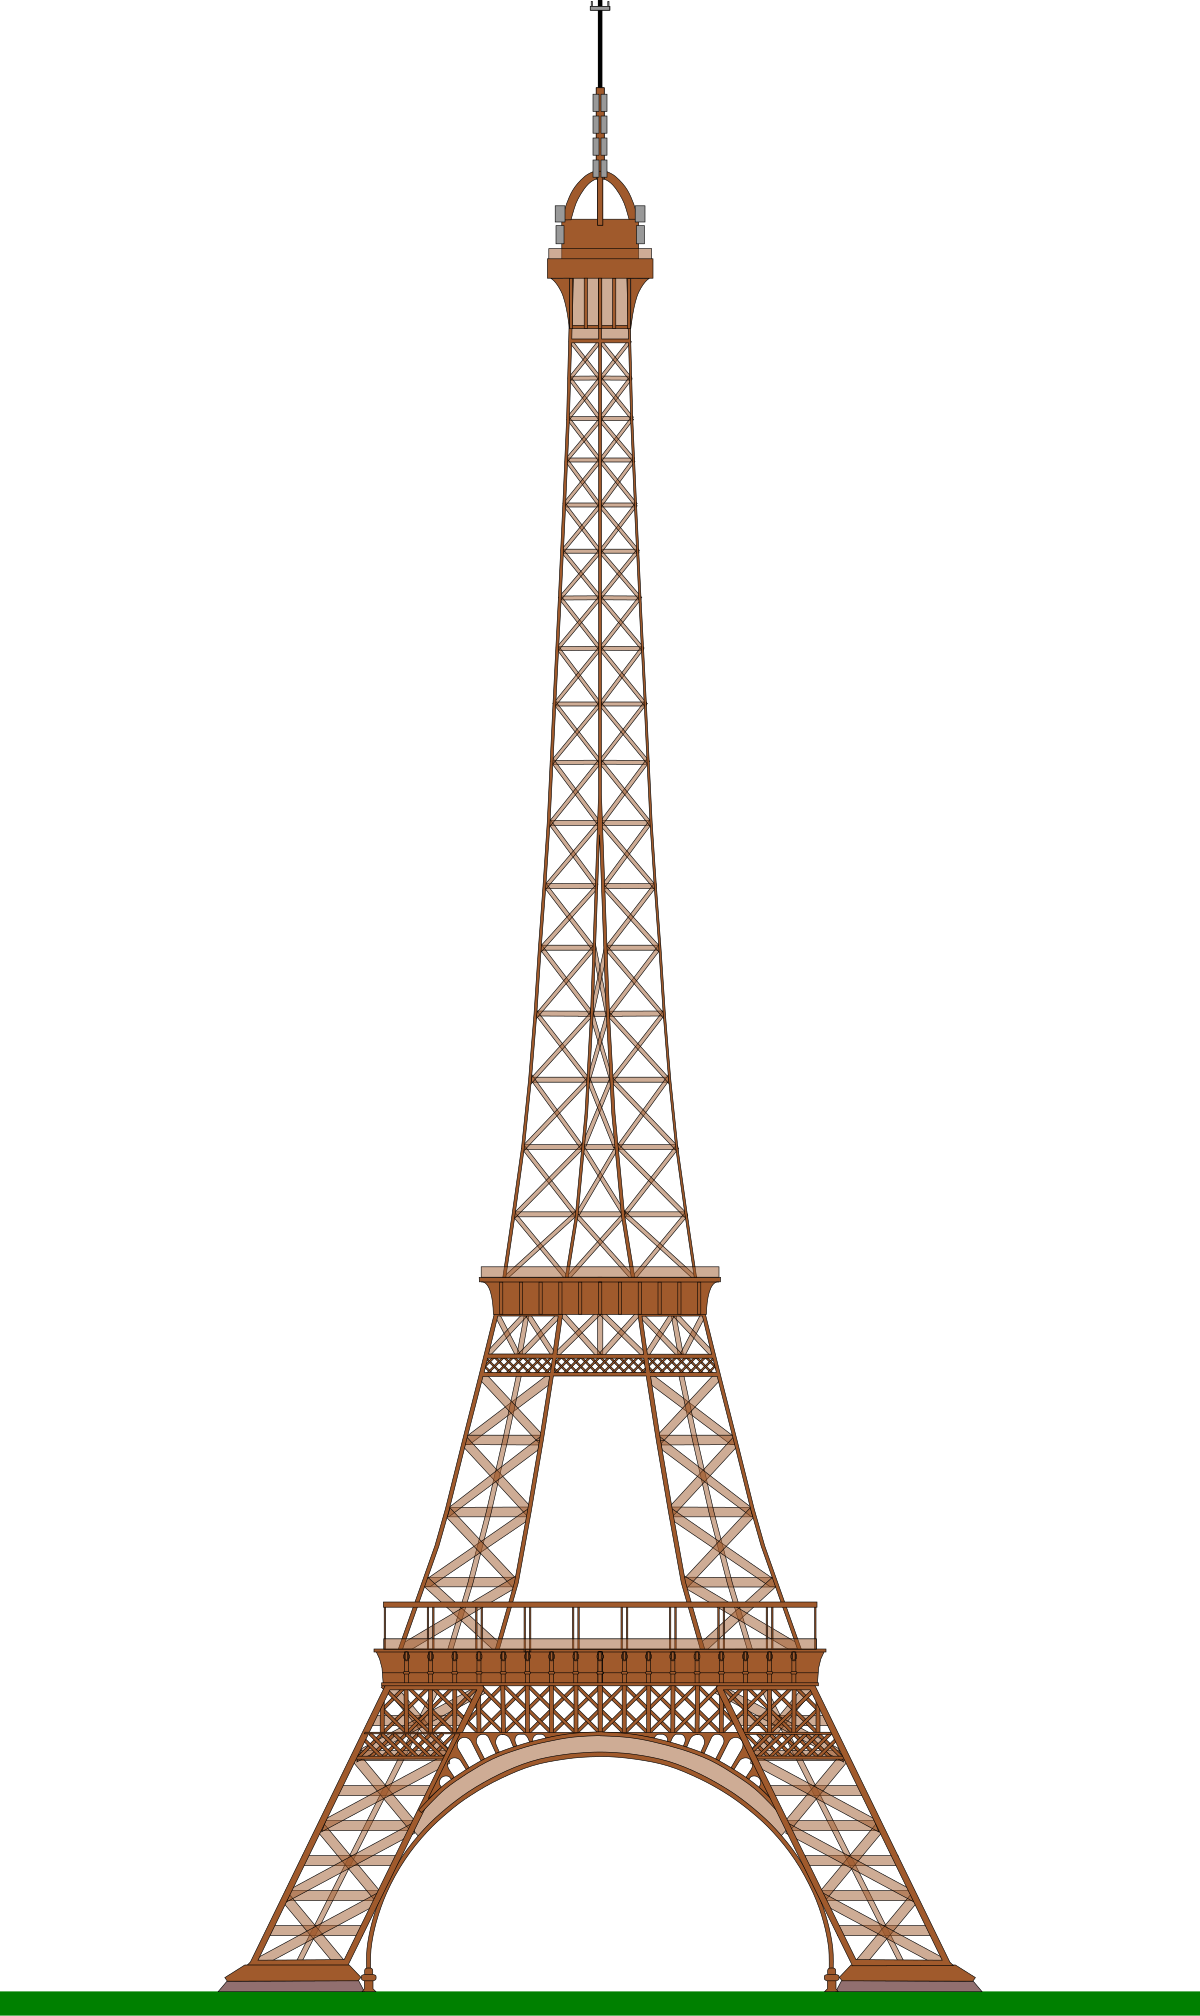
\includegraphics[scale=0.1]{Eiffel.png}};
	\draw[thick] ([shift={(0,-0.15)}]A.north) coordinate (A)--++(0,-7) coordinate (B)--+(3,0) coordinate (C)--cycle;
	\path ($(C)+(2,0)$) coordinate (D);
	\draw pic["$\alpha$",draw=violet, fill=yellow, angle radius = 10,thick, angle eccentricity = 1.5,font = \large] {angle = A--C--B}
	 pic["$\beta$",draw=violet, fill=teal!50, angle radius = 10,thick, angle eccentricity = 1.5,font = \large] {angle = A--D--B};
	 \draw[shift={(B)}] (0,0) rectangle (9pt,9pt);
	 \draw (B)--(D)--(A)--cycle;
	\foreach \p/\q in {A/80,B/-90,C/-90,D/-90} \draw[fill=white,line width=0.3pt] (\p) circle(1.5pt) node[shift={(\q:8pt)}]{\color{violet}$\p$};
\end{tikzpicture}
\end{document}